\documentclass{standalone}
\usepackage{tikz}
\begin{document}
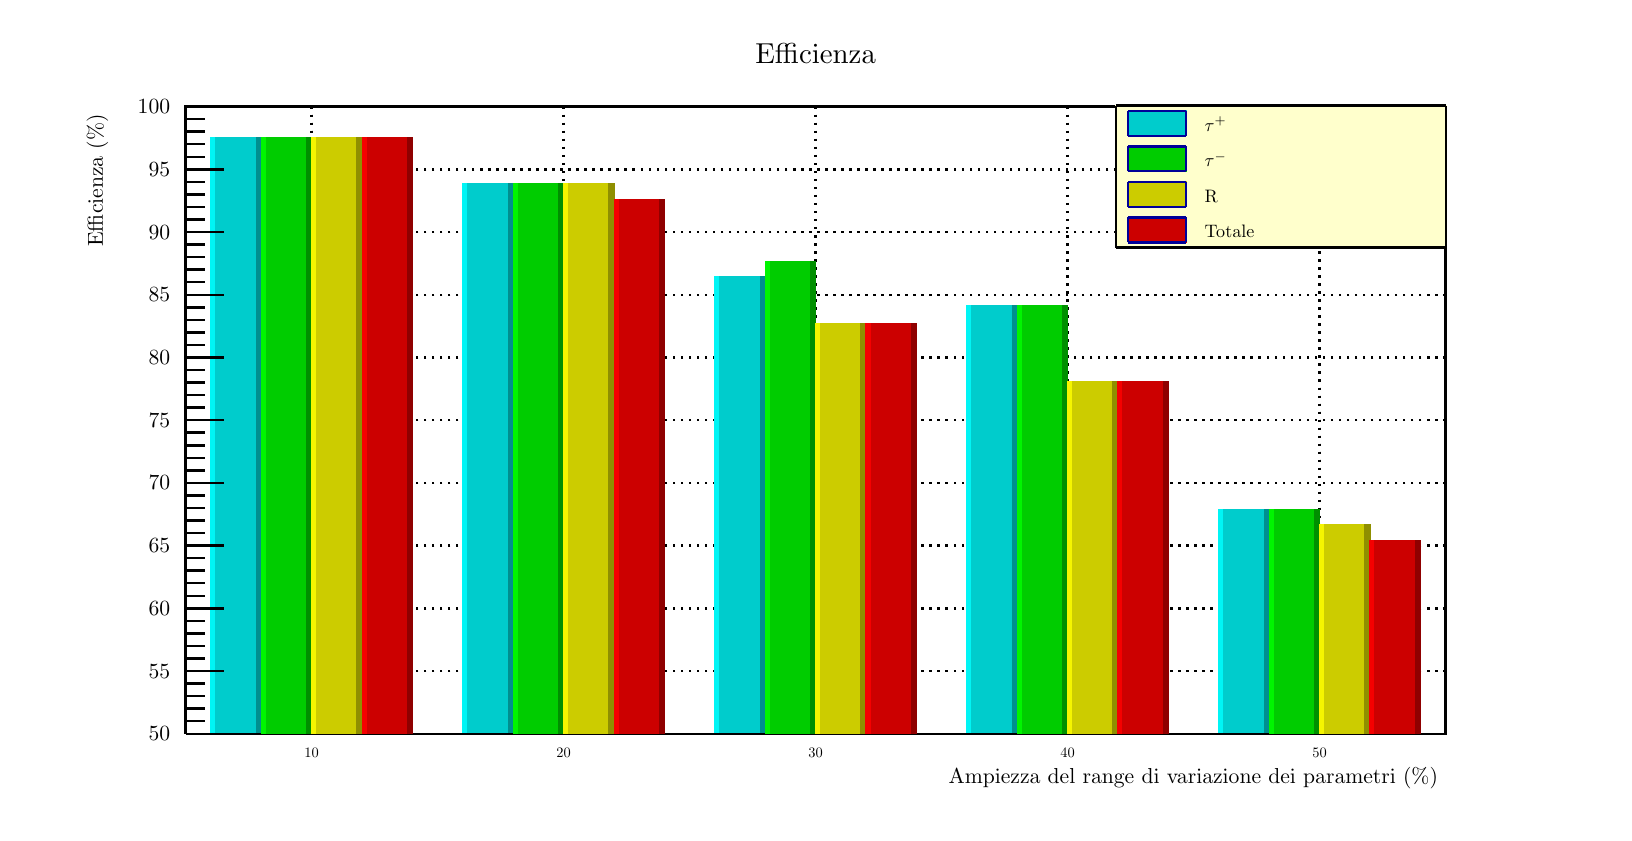
\begin{tikzpicture}
\pgfdeclareplotmark{cross} {
\pgfpathmoveto{\pgfpoint{-0.3\pgfplotmarksize}{\pgfplotmarksize}}
\pgfpathlineto{\pgfpoint{+0.3\pgfplotmarksize}{\pgfplotmarksize}}
\pgfpathlineto{\pgfpoint{+0.3\pgfplotmarksize}{0.3\pgfplotmarksize}}
\pgfpathlineto{\pgfpoint{+1\pgfplotmarksize}{0.3\pgfplotmarksize}}
\pgfpathlineto{\pgfpoint{+1\pgfplotmarksize}{-0.3\pgfplotmarksize}}
\pgfpathlineto{\pgfpoint{+0.3\pgfplotmarksize}{-0.3\pgfplotmarksize}}
\pgfpathlineto{\pgfpoint{+0.3\pgfplotmarksize}{-1.\pgfplotmarksize}}
\pgfpathlineto{\pgfpoint{-0.3\pgfplotmarksize}{-1.\pgfplotmarksize}}
\pgfpathlineto{\pgfpoint{-0.3\pgfplotmarksize}{-0.3\pgfplotmarksize}}
\pgfpathlineto{\pgfpoint{-1.\pgfplotmarksize}{-0.3\pgfplotmarksize}}
\pgfpathlineto{\pgfpoint{-1.\pgfplotmarksize}{0.3\pgfplotmarksize}}
\pgfpathlineto{\pgfpoint{-0.3\pgfplotmarksize}{0.3\pgfplotmarksize}}
\pgfpathclose
\pgfusepathqstroke
}
\pgfdeclareplotmark{cross*} {
\pgfpathmoveto{\pgfpoint{-0.3\pgfplotmarksize}{\pgfplotmarksize}}
\pgfpathlineto{\pgfpoint{+0.3\pgfplotmarksize}{\pgfplotmarksize}}
\pgfpathlineto{\pgfpoint{+0.3\pgfplotmarksize}{0.3\pgfplotmarksize}}
\pgfpathlineto{\pgfpoint{+1\pgfplotmarksize}{0.3\pgfplotmarksize}}
\pgfpathlineto{\pgfpoint{+1\pgfplotmarksize}{-0.3\pgfplotmarksize}}
\pgfpathlineto{\pgfpoint{+0.3\pgfplotmarksize}{-0.3\pgfplotmarksize}}
\pgfpathlineto{\pgfpoint{+0.3\pgfplotmarksize}{-1.\pgfplotmarksize}}
\pgfpathlineto{\pgfpoint{-0.3\pgfplotmarksize}{-1.\pgfplotmarksize}}
\pgfpathlineto{\pgfpoint{-0.3\pgfplotmarksize}{-0.3\pgfplotmarksize}}
\pgfpathlineto{\pgfpoint{-1.\pgfplotmarksize}{-0.3\pgfplotmarksize}}
\pgfpathlineto{\pgfpoint{-1.\pgfplotmarksize}{0.3\pgfplotmarksize}}
\pgfpathlineto{\pgfpoint{-0.3\pgfplotmarksize}{0.3\pgfplotmarksize}}
\pgfpathclose
\pgfusepathqfillstroke
}
\pgfdeclareplotmark{newstar} {
\pgfpathmoveto{\pgfqpoint{0pt}{\pgfplotmarksize}}
\pgfpathlineto{\pgfqpointpolar{44}{0.5\pgfplotmarksize}}
\pgfpathlineto{\pgfqpointpolar{18}{\pgfplotmarksize}}
\pgfpathlineto{\pgfqpointpolar{-20}{0.5\pgfplotmarksize}}
\pgfpathlineto{\pgfqpointpolar{-54}{\pgfplotmarksize}}
\pgfpathlineto{\pgfqpointpolar{-90}{0.5\pgfplotmarksize}}
\pgfpathlineto{\pgfqpointpolar{234}{\pgfplotmarksize}}
\pgfpathlineto{\pgfqpointpolar{198}{0.5\pgfplotmarksize}}
\pgfpathlineto{\pgfqpointpolar{162}{\pgfplotmarksize}}
\pgfpathlineto{\pgfqpointpolar{134}{0.5\pgfplotmarksize}}
\pgfpathclose
\pgfusepathqstroke
}
\pgfdeclareplotmark{newstar*} {
\pgfpathmoveto{\pgfqpoint{0pt}{\pgfplotmarksize}}
\pgfpathlineto{\pgfqpointpolar{44}{0.5\pgfplotmarksize}}
\pgfpathlineto{\pgfqpointpolar{18}{\pgfplotmarksize}}
\pgfpathlineto{\pgfqpointpolar{-20}{0.5\pgfplotmarksize}}
\pgfpathlineto{\pgfqpointpolar{-54}{\pgfplotmarksize}}
\pgfpathlineto{\pgfqpointpolar{-90}{0.5\pgfplotmarksize}}
\pgfpathlineto{\pgfqpointpolar{234}{\pgfplotmarksize}}
\pgfpathlineto{\pgfqpointpolar{198}{0.5\pgfplotmarksize}}
\pgfpathlineto{\pgfqpointpolar{162}{\pgfplotmarksize}}
\pgfpathlineto{\pgfqpointpolar{134}{0.5\pgfplotmarksize}}
\pgfpathclose
\pgfusepathqfillstroke
}
\definecolor{c}{rgb}{1,1,1};
\draw [color=c, fill=c] (0,0) rectangle (20,9.95601);
\draw [color=c, fill=c] (2,0.995601) rectangle (18,8.96041);
\definecolor{c}{rgb}{0,0,0};
\draw [c,line width=0.9] (2,0.995601) -- (2,8.96041) -- (18,8.96041) -- (18,0.995601) -- (2,0.995601);
\definecolor{c}{rgb}{1,1,1};
\draw [color=c, fill=c] (2,0.995601) rectangle (18,8.96041);
\definecolor{c}{rgb}{0,0,0};
\draw [c,line width=0.9] (2,0.995601) -- (2,8.96041) -- (18,8.96041) -- (18,0.995601) -- (2,0.995601);
\draw [c,line width=0.9] (2,0.995601) -- (18,0.995601);
\draw [c,dotted,line width=0.9] (3.6,8.96041) -- (3.6,0.995601);
\draw [c,dotted,line width=0.9] (6.8,8.96041) -- (6.8,0.995601);
\draw [c,dotted,line width=0.9] (10,8.96041) -- (10,0.995601);
\draw [c,dotted,line width=0.9] (13.2,8.96041) -- (13.2,0.995601);
\draw [c,dotted,line width=0.9] (16.4,8.96041) -- (16.4,0.995601);
\draw [c,dotted,line width=0.9] (3.6,8.96041) -- (3.6,0.995601);
\draw [c,dotted,line width=0.9] (16.4,8.96041) -- (16.4,0.995601);
\draw [c,line width=0.9] (2,0.995601) -- (2,8.96041);
\draw [c,dotted,line width=0.9] (18,0.995601) -- (2,0.995601);
\draw [c,dotted,line width=0.9] (18,1.79208) -- (2,1.79208);
\draw [c,dotted,line width=0.9] (18,2.58856) -- (2,2.58856);
\draw [c,dotted,line width=0.9] (18,3.38504) -- (2,3.38504);
\draw [c,dotted,line width=0.9] (18,4.18152) -- (2,4.18152);
\draw [c,dotted,line width=0.9] (18,4.97801) -- (2,4.97801);
\draw [c,dotted,line width=0.9] (18,5.77449) -- (2,5.77449);
\draw [c,dotted,line width=0.9] (18,6.57097) -- (2,6.57097);
\draw [c,dotted,line width=0.9] (18,7.36745) -- (2,7.36745);
\draw [c,dotted,line width=0.9] (18,8.16393) -- (2,8.16393);
\draw [c,dotted,line width=0.9] (18,8.96041) -- (2,8.96041);
\definecolor{c}{rgb}{0,0.96,0.96};
\draw [color=c, fill=c] (2.32,0.995601) rectangle (2.384,8.56709);
\definecolor{c}{rgb}{0,0.8,0.8};
\draw [color=c, fill=c] (2.384,0.995601) rectangle (2.896,8.56709);
\definecolor{c}{rgb}{0,0.56,0.56};
\draw [color=c, fill=c] (2.896,0.995601) rectangle (2.96,8.56709);
\definecolor{c}{rgb}{0,0.96,0.96};
\draw [color=c, fill=c] (5.52,0.995601) rectangle (5.584,7.97711);
\definecolor{c}{rgb}{0,0.8,0.8};
\draw [color=c, fill=c] (5.584,0.995601) rectangle (6.096,7.97711);
\definecolor{c}{rgb}{0,0.56,0.56};
\draw [color=c, fill=c] (6.096,0.995601) rectangle (6.16,7.97711);
\definecolor{c}{rgb}{0,0.96,0.96};
\draw [color=c, fill=c] (8.72,0.995601) rectangle (8.784,6.79714);
\definecolor{c}{rgb}{0,0.8,0.8};
\draw [color=c, fill=c] (8.784,0.995601) rectangle (9.296,6.79714);
\definecolor{c}{rgb}{0,0.56,0.56};
\draw [color=c, fill=c] (9.296,0.995601) rectangle (9.36,6.79714);
\definecolor{c}{rgb}{0,0.96,0.96};
\draw [color=c, fill=c] (11.92,0.995601) rectangle (11.984,6.43498);
\definecolor{c}{rgb}{0,0.8,0.8};
\draw [color=c, fill=c] (11.984,0.995601) rectangle (12.496,6.43498);
\definecolor{c}{rgb}{0,0.56,0.56};
\draw [color=c, fill=c] (12.496,0.995601) rectangle (12.56,6.43498);
\definecolor{c}{rgb}{0,0.96,0.96};
\draw [color=c, fill=c] (15.12,0.995601) rectangle (15.184,3.84719);
\definecolor{c}{rgb}{0,0.8,0.8};
\draw [color=c, fill=c] (15.184,0.995601) rectangle (15.696,3.84719);
\definecolor{c}{rgb}{0,0.56,0.56};
\draw [color=c, fill=c] (15.696,0.995601) rectangle (15.76,3.84719);
\definecolor{c}{rgb}{0,0,0};
\draw [c,line width=0.9] (2,0.995601) -- (18,0.995601);
\draw [anchor= east] (18,0.438065) node[scale=0.781573, color=c, rotate=0]{Ampiezza del range di variazione dei parametri (\%)};
\draw [anchor=north] (3.6,0.876129) node[scale=0.521049, color=c, rotate=0]{10};
\draw [anchor=north] (6.8,0.876129) node[scale=0.521049, color=c, rotate=0]{20};
\draw [anchor=north] (10,0.876129) node[scale=0.521049, color=c, rotate=0]{30};
\draw [anchor=north] (13.2,0.876129) node[scale=0.521049, color=c, rotate=0]{40};
\draw [anchor=north] (16.4,0.876129) node[scale=0.521049, color=c, rotate=0]{50};
\draw [c,line width=0.9] (3.6,1.23455) -- (3.6,0.995601);
\draw [c,line width=0.9] (6.8,1.23455) -- (6.8,0.995601);
\draw [c,line width=0.9] (10,1.23455) -- (10,0.995601);
\draw [c,line width=0.9] (13.2,1.23455) -- (13.2,0.995601);
\draw [c,line width=0.9] (16.4,1.23455) -- (16.4,0.995601);
\draw [c,line width=0.9] (3.6,1.23455) -- (3.6,0.995601);
\draw [c,line width=0.9] (16.4,1.23455) -- (16.4,0.995601);
\draw [c,line width=0.9] (2,0.995601) -- (2,8.96041);
\draw [anchor= east] (0.88,8.96041) node[scale=0.781573, color=c, rotate=90]{Efficienza (\%)};
\draw [c,line width=0.9] (2.48,0.995601) -- (2,0.995601);
\draw [c,line width=0.9] (2.24,1.1549) -- (2,1.1549);
\draw [c,line width=0.9] (2.24,1.31419) -- (2,1.31419);
\draw [c,line width=0.9] (2.24,1.47349) -- (2,1.47349);
\draw [c,line width=0.9] (2.24,1.63279) -- (2,1.63279);
\draw [c,line width=0.9] (2.48,1.79208) -- (2,1.79208);
\draw [c,line width=0.9] (2.24,1.95138) -- (2,1.95138);
\draw [c,line width=0.9] (2.24,2.11067) -- (2,2.11067);
\draw [c,line width=0.9] (2.24,2.26997) -- (2,2.26997);
\draw [c,line width=0.9] (2.24,2.42927) -- (2,2.42927);
\draw [c,line width=0.9] (2.48,2.58856) -- (2,2.58856);
\draw [c,line width=0.9] (2.24,2.74786) -- (2,2.74786);
\draw [c,line width=0.9] (2.24,2.90716) -- (2,2.90716);
\draw [c,line width=0.9] (2.24,3.06645) -- (2,3.06645);
\draw [c,line width=0.9] (2.24,3.22575) -- (2,3.22575);
\draw [c,line width=0.9] (2.48,3.38504) -- (2,3.38504);
\draw [c,line width=0.9] (2.24,3.54434) -- (2,3.54434);
\draw [c,line width=0.9] (2.24,3.70364) -- (2,3.70364);
\draw [c,line width=0.9] (2.24,3.86293) -- (2,3.86293);
\draw [c,line width=0.9] (2.24,4.02223) -- (2,4.02223);
\draw [c,line width=0.9] (2.48,4.18152) -- (2,4.18152);
\draw [c,line width=0.9] (2.24,4.34082) -- (2,4.34082);
\draw [c,line width=0.9] (2.24,4.50012) -- (2,4.50012);
\draw [c,line width=0.9] (2.24,4.65941) -- (2,4.65941);
\draw [c,line width=0.9] (2.24,4.81871) -- (2,4.81871);
\draw [c,line width=0.9] (2.48,4.97801) -- (2,4.97801);
\draw [c,line width=0.9] (2.24,5.1373) -- (2,5.1373);
\draw [c,line width=0.9] (2.24,5.2966) -- (2,5.2966);
\draw [c,line width=0.9] (2.24,5.45589) -- (2,5.45589);
\draw [c,line width=0.9] (2.24,5.61519) -- (2,5.61519);
\draw [c,line width=0.9] (2.48,5.77449) -- (2,5.77449);
\draw [c,line width=0.9] (2.24,5.93378) -- (2,5.93378);
\draw [c,line width=0.9] (2.24,6.09308) -- (2,6.09308);
\draw [c,line width=0.9] (2.24,6.25238) -- (2,6.25238);
\draw [c,line width=0.9] (2.24,6.41167) -- (2,6.41167);
\draw [c,line width=0.9] (2.48,6.57097) -- (2,6.57097);
\draw [c,line width=0.9] (2.24,6.73026) -- (2,6.73026);
\draw [c,line width=0.9] (2.24,6.88956) -- (2,6.88956);
\draw [c,line width=0.9] (2.24,7.04886) -- (2,7.04886);
\draw [c,line width=0.9] (2.24,7.20815) -- (2,7.20815);
\draw [c,line width=0.9] (2.48,7.36745) -- (2,7.36745);
\draw [c,line width=0.9] (2.24,7.52674) -- (2,7.52674);
\draw [c,line width=0.9] (2.24,7.68604) -- (2,7.68604);
\draw [c,line width=0.9] (2.24,7.84534) -- (2,7.84534);
\draw [c,line width=0.9] (2.24,8.00463) -- (2,8.00463);
\draw [c,line width=0.9] (2.48,8.16393) -- (2,8.16393);
\draw [c,line width=0.9] (2.24,8.32323) -- (2,8.32323);
\draw [c,line width=0.9] (2.24,8.48252) -- (2,8.48252);
\draw [c,line width=0.9] (2.24,8.64182) -- (2,8.64182);
\draw [c,line width=0.9] (2.24,8.80111) -- (2,8.80111);
\draw [c,line width=0.9] (2.48,8.96041) -- (2,8.96041);
\draw [anchor= east] (1.9,0.995601) node[scale=0.781573, color=c, rotate=0]{50};
\draw [anchor= east] (1.9,1.79208) node[scale=0.781573, color=c, rotate=0]{55};
\draw [anchor= east] (1.9,2.58856) node[scale=0.781573, color=c, rotate=0]{60};
\draw [anchor= east] (1.9,3.38504) node[scale=0.781573, color=c, rotate=0]{65};
\draw [anchor= east] (1.9,4.18152) node[scale=0.781573, color=c, rotate=0]{70};
\draw [anchor= east] (1.9,4.97801) node[scale=0.781573, color=c, rotate=0]{75};
\draw [anchor= east] (1.9,5.77449) node[scale=0.781573, color=c, rotate=0]{80};
\draw [anchor= east] (1.9,6.57097) node[scale=0.781573, color=c, rotate=0]{85};
\draw [anchor= east] (1.9,7.36745) node[scale=0.781573, color=c, rotate=0]{90};
\draw [anchor= east] (1.9,8.16393) node[scale=0.781573, color=c, rotate=0]{95};
\draw [anchor= east] (1.9,8.96041) node[scale=0.781573, color=c, rotate=0]{100};
\definecolor{c}{rgb}{0,0.96,0};
\draw [color=c, fill=c] (2.96,0.995601) rectangle (3.024,8.56709);
\definecolor{c}{rgb}{0,0.8,0};
\draw [color=c, fill=c] (3.024,0.995601) rectangle (3.536,8.56709);
\definecolor{c}{rgb}{0,0.56,0};
\draw [color=c, fill=c] (3.536,0.995601) rectangle (3.6,8.56709);
\definecolor{c}{rgb}{0,0.96,0};
\draw [color=c, fill=c] (6.16,0.995601) rectangle (6.224,7.97711);
\definecolor{c}{rgb}{0,0.8,0};
\draw [color=c, fill=c] (6.224,0.995601) rectangle (6.736,7.97711);
\definecolor{c}{rgb}{0,0.56,0};
\draw [color=c, fill=c] (6.736,0.995601) rectangle (6.8,7.97711);
\definecolor{c}{rgb}{0,0.96,0};
\draw [color=c, fill=c] (9.36,0.995601) rectangle (9.424,6.99379);
\definecolor{c}{rgb}{0,0.8,0};
\draw [color=c, fill=c] (9.424,0.995601) rectangle (9.936,6.99379);
\definecolor{c}{rgb}{0,0.56,0};
\draw [color=c, fill=c] (9.936,0.995601) rectangle (10,6.99379);
\definecolor{c}{rgb}{0,0.96,0};
\draw [color=c, fill=c] (12.56,0.995601) rectangle (12.624,6.43498);
\definecolor{c}{rgb}{0,0.8,0};
\draw [color=c, fill=c] (12.624,0.995601) rectangle (13.136,6.43498);
\definecolor{c}{rgb}{0,0.56,0};
\draw [color=c, fill=c] (13.136,0.995601) rectangle (13.2,6.43498);
\definecolor{c}{rgb}{0,0.96,0};
\draw [color=c, fill=c] (15.76,0.995601) rectangle (15.824,3.84719);
\definecolor{c}{rgb}{0,0.8,0};
\draw [color=c, fill=c] (15.824,0.995601) rectangle (16.336,3.84719);
\definecolor{c}{rgb}{0,0.56,0};
\draw [color=c, fill=c] (16.336,0.995601) rectangle (16.4,3.84719);
\definecolor{c}{rgb}{0.96,0.96,0};
\draw [color=c, fill=c] (3.6,0.995601) rectangle (3.664,8.56709);
\definecolor{c}{rgb}{0.8,0.8,0};
\draw [color=c, fill=c] (3.664,0.995601) rectangle (4.176,8.56709);
\definecolor{c}{rgb}{0.56,0.56,0};
\draw [color=c, fill=c] (4.176,0.995601) rectangle (4.24,8.56709);
\definecolor{c}{rgb}{0.96,0.96,0};
\draw [color=c, fill=c] (6.8,0.995601) rectangle (6.864,7.97711);
\definecolor{c}{rgb}{0.8,0.8,0};
\draw [color=c, fill=c] (6.864,0.995601) rectangle (7.376,7.97711);
\definecolor{c}{rgb}{0.56,0.56,0};
\draw [color=c, fill=c] (7.376,0.995601) rectangle (7.44,7.97711);
\definecolor{c}{rgb}{0.96,0.96,0};
\draw [color=c, fill=c] (10,0.995601) rectangle (10.064,6.20714);
\definecolor{c}{rgb}{0.8,0.8,0};
\draw [color=c, fill=c] (10.064,0.995601) rectangle (10.576,6.20714);
\definecolor{c}{rgb}{0.56,0.56,0};
\draw [color=c, fill=c] (10.576,0.995601) rectangle (10.64,6.20714);
\definecolor{c}{rgb}{0.96,0.96,0};
\draw [color=c, fill=c] (13.2,0.995601) rectangle (13.264,5.46367);
\definecolor{c}{rgb}{0.8,0.8,0};
\draw [color=c, fill=c] (13.264,0.995601) rectangle (13.776,5.46367);
\definecolor{c}{rgb}{0.56,0.56,0};
\draw [color=c, fill=c] (13.776,0.995601) rectangle (13.84,5.46367);
\definecolor{c}{rgb}{0.96,0.96,0};
\draw [color=c, fill=c] (16.4,0.995601) rectangle (16.464,3.65054);
\definecolor{c}{rgb}{0.8,0.8,0};
\draw [color=c, fill=c] (16.464,0.995601) rectangle (16.976,3.65054);
\definecolor{c}{rgb}{0.56,0.56,0};
\draw [color=c, fill=c] (16.976,0.995601) rectangle (17.04,3.65054);
\definecolor{c}{rgb}{0.96,0,0};
\draw [color=c, fill=c] (4.24,0.995601) rectangle (4.304,8.56709);
\definecolor{c}{rgb}{0.8,0,0};
\draw [color=c, fill=c] (4.304,0.995601) rectangle (4.816,8.56709);
\definecolor{c}{rgb}{0.56,0,0};
\draw [color=c, fill=c] (4.816,0.995601) rectangle (4.88,8.56709);
\definecolor{c}{rgb}{0.96,0,0};
\draw [color=c, fill=c] (7.44,0.995601) rectangle (7.504,7.78044);
\definecolor{c}{rgb}{0.8,0,0};
\draw [color=c, fill=c] (7.504,0.995601) rectangle (8.016,7.78044);
\definecolor{c}{rgb}{0.56,0,0};
\draw [color=c, fill=c] (8.016,0.995601) rectangle (8.08,7.78044);
\definecolor{c}{rgb}{0.96,0,0};
\draw [color=c, fill=c] (10.64,0.995601) rectangle (10.704,6.20714);
\definecolor{c}{rgb}{0.8,0,0};
\draw [color=c, fill=c] (10.704,0.995601) rectangle (11.216,6.20714);
\definecolor{c}{rgb}{0.56,0,0};
\draw [color=c, fill=c] (11.216,0.995601) rectangle (11.28,6.20714);
\definecolor{c}{rgb}{0.96,0,0};
\draw [color=c, fill=c] (13.84,0.995601) rectangle (13.904,5.46367);
\definecolor{c}{rgb}{0.8,0,0};
\draw [color=c, fill=c] (13.904,0.995601) rectangle (14.416,5.46367);
\definecolor{c}{rgb}{0.56,0,0};
\draw [color=c, fill=c] (14.416,0.995601) rectangle (14.48,5.46367);
\definecolor{c}{rgb}{0.96,0,0};
\draw [color=c, fill=c] (17.04,0.995601) rectangle (17.104,3.45388);
\definecolor{c}{rgb}{0.8,0,0};
\draw [color=c, fill=c] (17.104,0.995601) rectangle (17.616,3.45388);
\definecolor{c}{rgb}{0.56,0,0};
\draw [color=c, fill=c] (17.616,0.995601) rectangle (17.68,3.45388);
\definecolor{c}{rgb}{1,1,0.8};
\draw [color=c, fill=c] (13.8123,7.17009) rectangle (18.0059,8.97361);
\definecolor{c}{rgb}{0,0,0};
\draw [c,line width=0.9] (13.8123,7.17009) -- (18.0059,7.17009);
\draw [c,line width=0.9] (18.0059,7.17009) -- (18.0059,8.97361);
\draw [c,line width=0.9] (18.0059,8.97361) -- (13.8123,8.97361);
\draw [c,line width=0.9] (13.8123,8.97361) -- (13.8123,7.17009);
\draw [anchor=base west] (14.8607,8.64672) node[scale=0.651311, color=c, rotate=0]{$\tau^{+}$};
\definecolor{c}{rgb}{0,0.8,0.8};
\draw [c, fill=c] (13.9696,8.59036) -- (14.7034,8.59036) -- (14.7034,8.90598) -- (13.9696,8.90598);
\definecolor{c}{rgb}{0,0,0.6};
\draw [c,line width=0.9] (13.9696,8.90598) -- (14.7034,8.90598);
\draw [c,line width=0.9] (13.9696,8.59036) -- (14.7034,8.59036);
\draw [c,line width=0.9] (14.7034,8.59036) -- (14.7034,8.90598);
\draw [c,line width=0.9] (13.9696,8.59036) -- (13.9696,8.90598);
\definecolor{c}{rgb}{0,0,0};
\draw [anchor=base west] (14.8607,8.19584) node[scale=0.651311, color=c, rotate=0]{$\tau^{-}$};
\definecolor{c}{rgb}{0,0.8,0};
\draw [c, fill=c] (13.9696,8.13948) -- (14.7034,8.13948) -- (14.7034,8.4551) -- (13.9696,8.4551);
\definecolor{c}{rgb}{0,0,0.6};
\draw [c,line width=0.9] (13.9696,8.4551) -- (14.7034,8.4551);
\draw [c,line width=0.9] (13.9696,8.13948) -- (14.7034,8.13948);
\draw [c,line width=0.9] (14.7034,8.13948) -- (14.7034,8.4551);
\draw [c,line width=0.9] (13.9696,8.13948) -- (13.9696,8.4551);
\definecolor{c}{rgb}{0,0,0};
\draw [anchor=base west] (14.8607,7.74496) node[scale=0.651311, color=c, rotate=0]{R};
\definecolor{c}{rgb}{0.8,0.8,0};
\draw [c, fill=c] (13.9696,7.6886) -- (14.7034,7.6886) -- (14.7034,8.00422) -- (13.9696,8.00422);
\definecolor{c}{rgb}{0,0,0.6};
\draw [c,line width=0.9] (13.9696,8.00422) -- (14.7034,8.00422);
\draw [c,line width=0.9] (13.9696,7.6886) -- (14.7034,7.6886);
\draw [c,line width=0.9] (14.7034,7.6886) -- (14.7034,8.00422);
\draw [c,line width=0.9] (13.9696,7.6886) -- (13.9696,8.00422);
\definecolor{c}{rgb}{0,0,0};
\draw [anchor=base west] (14.8607,7.29408) node[scale=0.651311, color=c, rotate=0]{Totale};
\definecolor{c}{rgb}{0.8,0,0};
\draw [c, fill=c] (13.9696,7.23772) -- (14.7034,7.23772) -- (14.7034,7.55334) -- (13.9696,7.55334);
\definecolor{c}{rgb}{0,0,0.6};
\draw [c,line width=0.9] (13.9696,7.55334) -- (14.7034,7.55334);
\draw [c,line width=0.9] (13.9696,7.23772) -- (14.7034,7.23772);
\draw [c,line width=0.9] (14.7034,7.23772) -- (14.7034,7.55334);
\draw [c,line width=0.9] (13.9696,7.23772) -- (13.9696,7.55334);
\definecolor{c}{rgb}{0,0,0};
\draw (10,9.63244) node[scale=1.0421, color=c, rotate=0]{Efficienza};
\end{tikzpicture}
\end{document}
